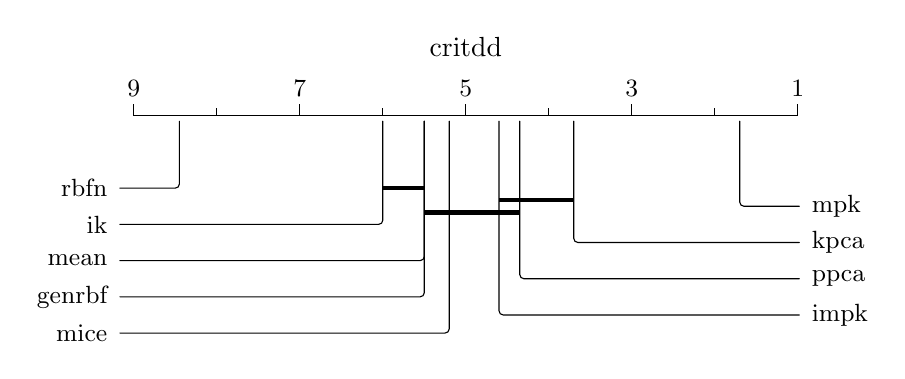
\begin{tikzpicture}[
  treatment line/.style={rounded corners=1.5pt, line cap=round, shorten >=1pt},
  treatment label/.style={font=\small},
  group line/.style={ultra thick},
]

\begin{axis}[
  clip={false},
  axis x line={center},
  axis y line={none},
  axis line style={-},
  xmin={1},
  ymax={0},
  scale only axis={true},
  width={\axisdefaultwidth},
  ticklabel style={anchor=south, yshift=1.3*\pgfkeysvalueof{/pgfplots/major tick length}, font=\small},
  every tick/.style={draw=black},
  major tick style={yshift=.5*\pgfkeysvalueof{/pgfplots/major tick length}},
  minor tick style={yshift=.5*\pgfkeysvalueof{/pgfplots/minor tick length}},
  title style={yshift=\baselineskip},
  xmax={9},
  ymin={-5.5},
  height={6\baselineskip},
  xtick={1,3,5,7,9},
  minor x tick num={1},
  x dir={reverse},
  title={critdd},
]

\draw[treatment line] ([yshift=-2pt] axis cs:1.7, 0) |- (axis cs:0.95, -2.5)
  node[treatment label, anchor=west] {mpk};
\draw[treatment line] ([yshift=-2pt] axis cs:3.7, 0) |- (axis cs:0.95, -3.5)
  node[treatment label, anchor=west] {kpca};
\draw[treatment line] ([yshift=-2pt] axis cs:4.35, 0) |- (axis cs:0.95, -4.5)
  node[treatment label, anchor=west] {ppca};
\draw[treatment line] ([yshift=-2pt] axis cs:4.6, 0) |- (axis cs:0.95, -5.5)
  node[treatment label, anchor=west] {impk};
\draw[treatment line] ([yshift=-2pt] axis cs:5.2, 0) |- (axis cs:9.2, -6.0)
  node[treatment label, anchor=east] {mice};
\draw[treatment line] ([yshift=-2pt] axis cs:5.5, 0) |- (axis cs:9.2, -5.0)
  node[treatment label, anchor=east] {genrbf};
\draw[treatment line] ([yshift=-2pt] axis cs:5.5, 0) |- (axis cs:9.2, -4.0)
  node[treatment label, anchor=east] {mean};
\draw[treatment line] ([yshift=-2pt] axis cs:6.0, 0) |- (axis cs:9.2, -3.0)
  node[treatment label, anchor=east] {ik};
\draw[treatment line] ([yshift=-2pt] axis cs:8.45, 0) |- (axis cs:9.2, -2.0)
  node[treatment label, anchor=east] {rbfn};
\draw[group line] (axis cs:5.5, -2.0) -- (axis cs:6.0, -2.0);
\draw[group line] (axis cs:4.35, -2.6666666666666665) -- (axis cs:5.5, -2.6666666666666665);
\draw[group line] (axis cs:3.7, -2.3333333333333335) -- (axis cs:4.6, -2.3333333333333335);

\end{axis}
\end{tikzpicture}